\documentclass[journal,12pt,twocolumn]{IEEEtran}
\usepackage[utf8]{inputenc}
\usepackage{amsmath}
\usepackage{amssymb}
\usepackage{tcolorbox}

\title{Assignment-4}
\author{Adepu Vasisht}
\date{CS20BTECH11002}
\providecommand{\brak}[1]{\ensuremath{\left(#1\right)}}
\begin{document}

\maketitle
\section*{GATE 2021(ST) Q.No 16}
Let $X$ be a random variable having distribution function 
\begin{equation}
\nonumber F(x)=
\begin{cases}
0, \quad x<1\\
\frac{a}{2}, \quad  1\leq x<2\\
\frac{c}{6}, \quad 2\leq x<3\\
1, \quad x\geq3
\end{cases}
\end{equation}
where $a$ and $c$ are appropriate constants. Let\\$A_n = \left[1+\frac{1}{n},3-\frac{1}{n}\right]$, $n\geq1$, and $A = \bigcup_{i=1}^{\infty}A_i$. If $\Pr\brak{X\leq1} = \frac{1}{2}$ and $E\brak{X} = \frac{5}{3}$, then $\Pr\brak{X\in A}$ equals to?

\section*{Solution}
\subsection{Proving that $X$ is a discrete variable}
To prove the above statement we plot $F\brak{x}$ which is the c.d.f of our random variable $X$ by taking some arbitrary values for $a$ and $c$ as it is mentioned that $a$ and $c$ are appropirate constants. The graph will be as shown in the figure below. 


\begin{figure}[h]
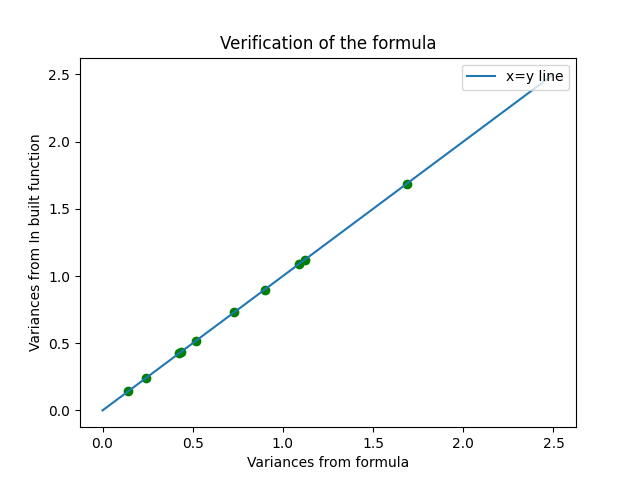
\includegraphics[scale=0.6]{ogimage}
\end{figure}

As we can see the graph is step-wise which means $X$ is a discrete random variable, moreover we can see that turns take place for $x=1,2,3$ so $X$ can take only these values.
\subsection{Finding $a$ and $c$}

So $X$ can take only 3 values namely 1,2 and 3.
Since we know that 
\begin{align}
 F\brak{1} &= \frac{a}{2}\\
\nonumber \\
 \Pr\brak{X\leq1} &= \frac{1}{2}\\
\nonumber \\
 \implies\frac{a}{2} &= \frac{1}{2}
\end{align}
 We calculate the value of $c$ using the given expectation value. The formula for a discrete variable is given by. 
$$E\brak{X} = \sum_{i=1}^{3}\Pr\brak{X=i}\cdot i$$

Since $X$ is a discrete random variable we have $\Pr\brak{X=1} = \Pr\brak{X\leq1} = \frac{1}{2}$\\And also since $F\brak{x}$ is a cdf we have $F\brak{2} = \Pr\brak{X=1}+\Pr\brak{X=2}$\\
$$\implies \Pr\brak{X=2} = \frac{c}{6}-\frac{1}{2}$$
Similarly we can say that $F\brak{3} = F\brak{2} + \Pr\brak{X=3}$
$$\implies \Pr\brak{X=3} = 1 - \frac{c}{6}$$
We have all the required probability values.
\begin{align}
 E\brak{X} &= \sum_{i=1}^{3}\Pr\brak{X=i}\cdot i\\
\nonumber \\
 &= \Pr\brak{1}.1 +2\Pr\brak{2} + 3\Pr\brak{3}\\
\nonumber \\
 &= \frac{1}{2}+ 2\brak{\frac{c}{6}-\frac{1}{2}}+3\brak{1-\frac{c}{6}}\\
\nonumber \\
\frac{5}{3} &= \frac{5}{2} - \frac{c}{6}\\
\nonumber \\
 \implies\frac{c}{6} &= \frac{5}{6}\\
\nonumber \\
 \therefore c &= 5
\end{align}



\subsection{Finding the range of A}
Given that $A_n = \left[1+\frac{1}{n},3-\frac{1}{n}\right]$, $n\geq1$, and \\$A = \bigcup_{i=1}^{\infty}A_i$. We can see  that for any i we have $A_i \subset A_{i+1}$ and we also know the property that if $A$ is a subset of $B$ then we have $$A\cup B = B$$\\\\
By applying the above principal we get that $A = A_\infty$ and since when $n \rightarrow \infty \implies \frac{1}{n} \rightarrow 0$ but not equal to 0 so we have $A = A_\infty = \brak{1,3}$

\subsection{Finding the probability }
 We know that $X$ can only take $X =1,2 \: \text{and}\: 3 $ as values and $A = \brak{1,3} $ hence the only value $X$ can take in $A$ is 2. We have $\Pr\brak{X\in A} = \Pr\brak{X = 2}$. And we know that  
\begin{align}
 \Pr\brak{X =2 } &= F\brak{2}-F\brak{1} \quad \brak{\because X \text{is discrete}}\\
\nonumber \\
\Pr\brak{X =2 } &= \frac{5}{6}-\frac{1}{2} \quad \brak{\because c =5 \,\text{and} \,a = 1}\\
\nonumber\\
 \implies \Pr\brak{X = 2} &= \frac{1}{3}=0.33
\end{align}

\end{document}